%-----------------------------------------------------------
%   Capítulo 7 - Resultados
%-----------------------------------------------------------
\chapter{Resultados}

Neste capítulo vão ser discutidos os resultados obtidos e os diferentes protótipos implementados.
\\Inicialmente para teste da leitura dos sensores e envio dos dados para o \textit{master}, foi tudo testado na \textit{breadboard}, como é possível ver na figura \ref{test}.

\begin{figure}[!htb]
\centering
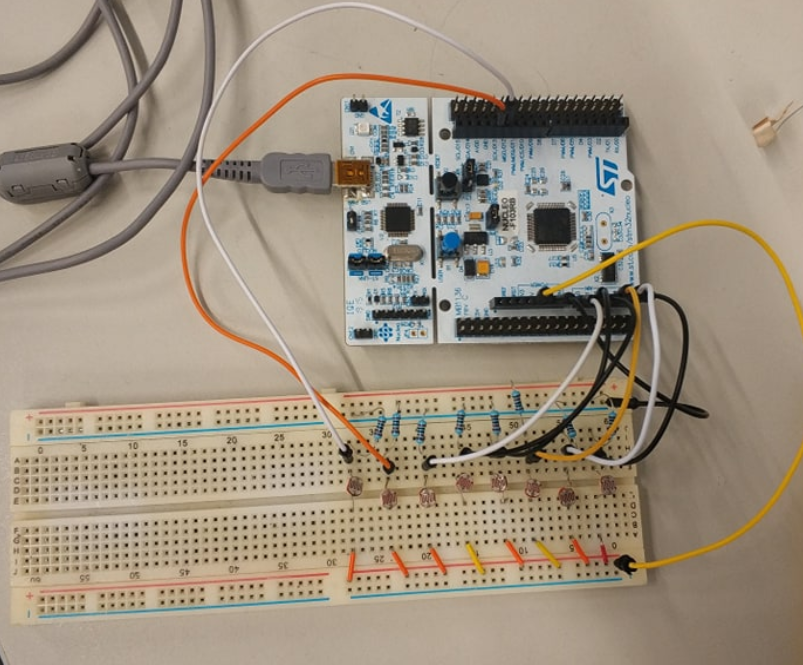
\includegraphics[scale=0.35]{Figuras/test.PNG}
\caption{Primeiro teste}
\label{test}
\end{figure}

Na figura \ref{anel} está representado o \textit{hardware} de um único na sua forma final.

\begin{figure}[!htb]
\centering
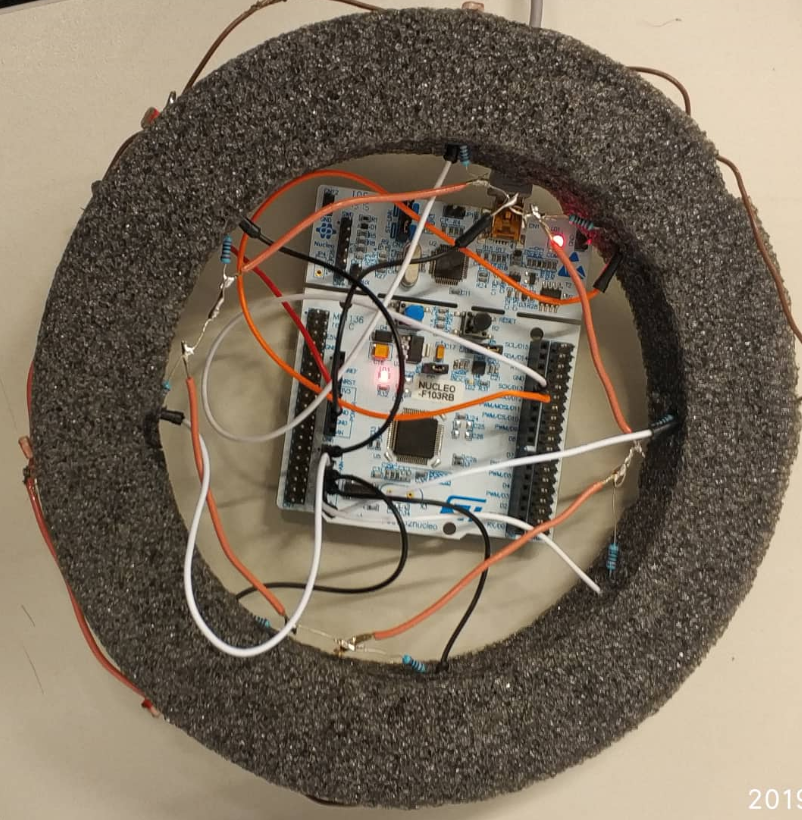
\includegraphics[scale=0.35]{Figuras/anel.PNG}
\caption{Circuito já implementado no anel}
\label{anel}
\end{figure}

\newpage
Na figura \ref{anel_final} está representado o \textit{hardware} com todos os anéis prontos para a comunicar.

\begin{figure}[!htb]
\centering
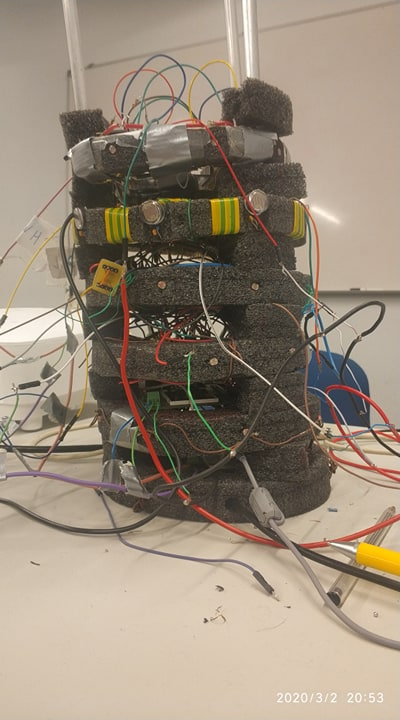
\includegraphics[scale=0.35]{Figuras/anel_final.jpg}
\caption{Protótipo na sua forma final}
\label{anel_final}
\end{figure}



\newpage
Nas figuras \ref{1} e \ref{2} está a comparação de dois algoritmos (infelizmente não foi  feita a suavização dos gráficos) que foram testados para o calculo do roll, para o teste foi dada uma volta de 360º com o anel, como é possível observar na figura do lado esquerdo obtém-se melhores resultados em relação à figura direito, em que parece que o roll é obtido às partes.
\\Portanto o algoritmo escolhido foi o da figura do lado esquerdo, pois os resultados são muito mais decentes.

\begin{figure}[!tbp]
  \centering
  \begin{minipage}[b]{0.45\textwidth}
    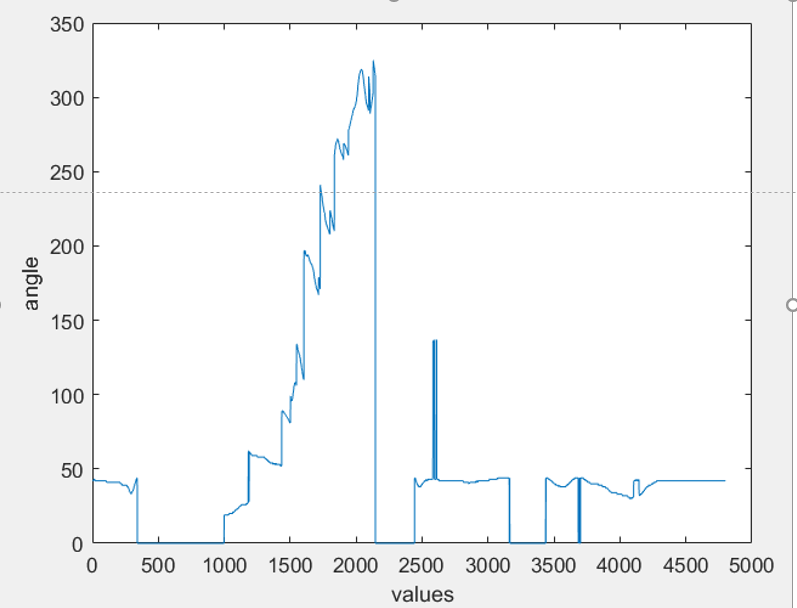
\includegraphics[width=\textwidth]{Figuras/alg1.PNG}
    \caption{Algoritmo 1}
    \label{1}
  \end{minipage}
  \hfill
  \begin{minipage}[b]{0.45\textwidth}
    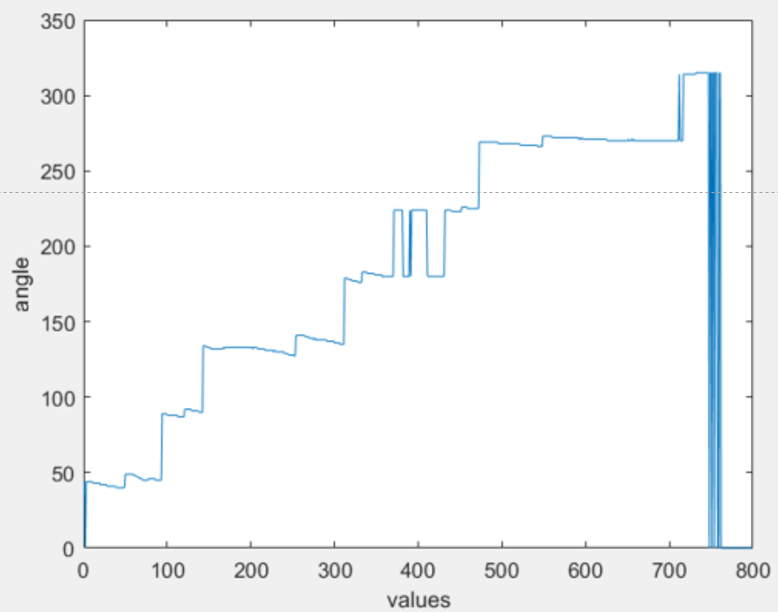
\includegraphics[width=\textwidth]{Figuras/alg2.PNG}
    \caption{Algoritmo 2}
    \label{2}
  \end{minipage}
  
\end{figure}

Na figura \ref{todos} está o resultado com todos os anéis a comunicar, nos primeiros 1500 valores lidos foi dado uma volta de 360 graus em torno do anel.
\begin{figure}[!htb]
\centering
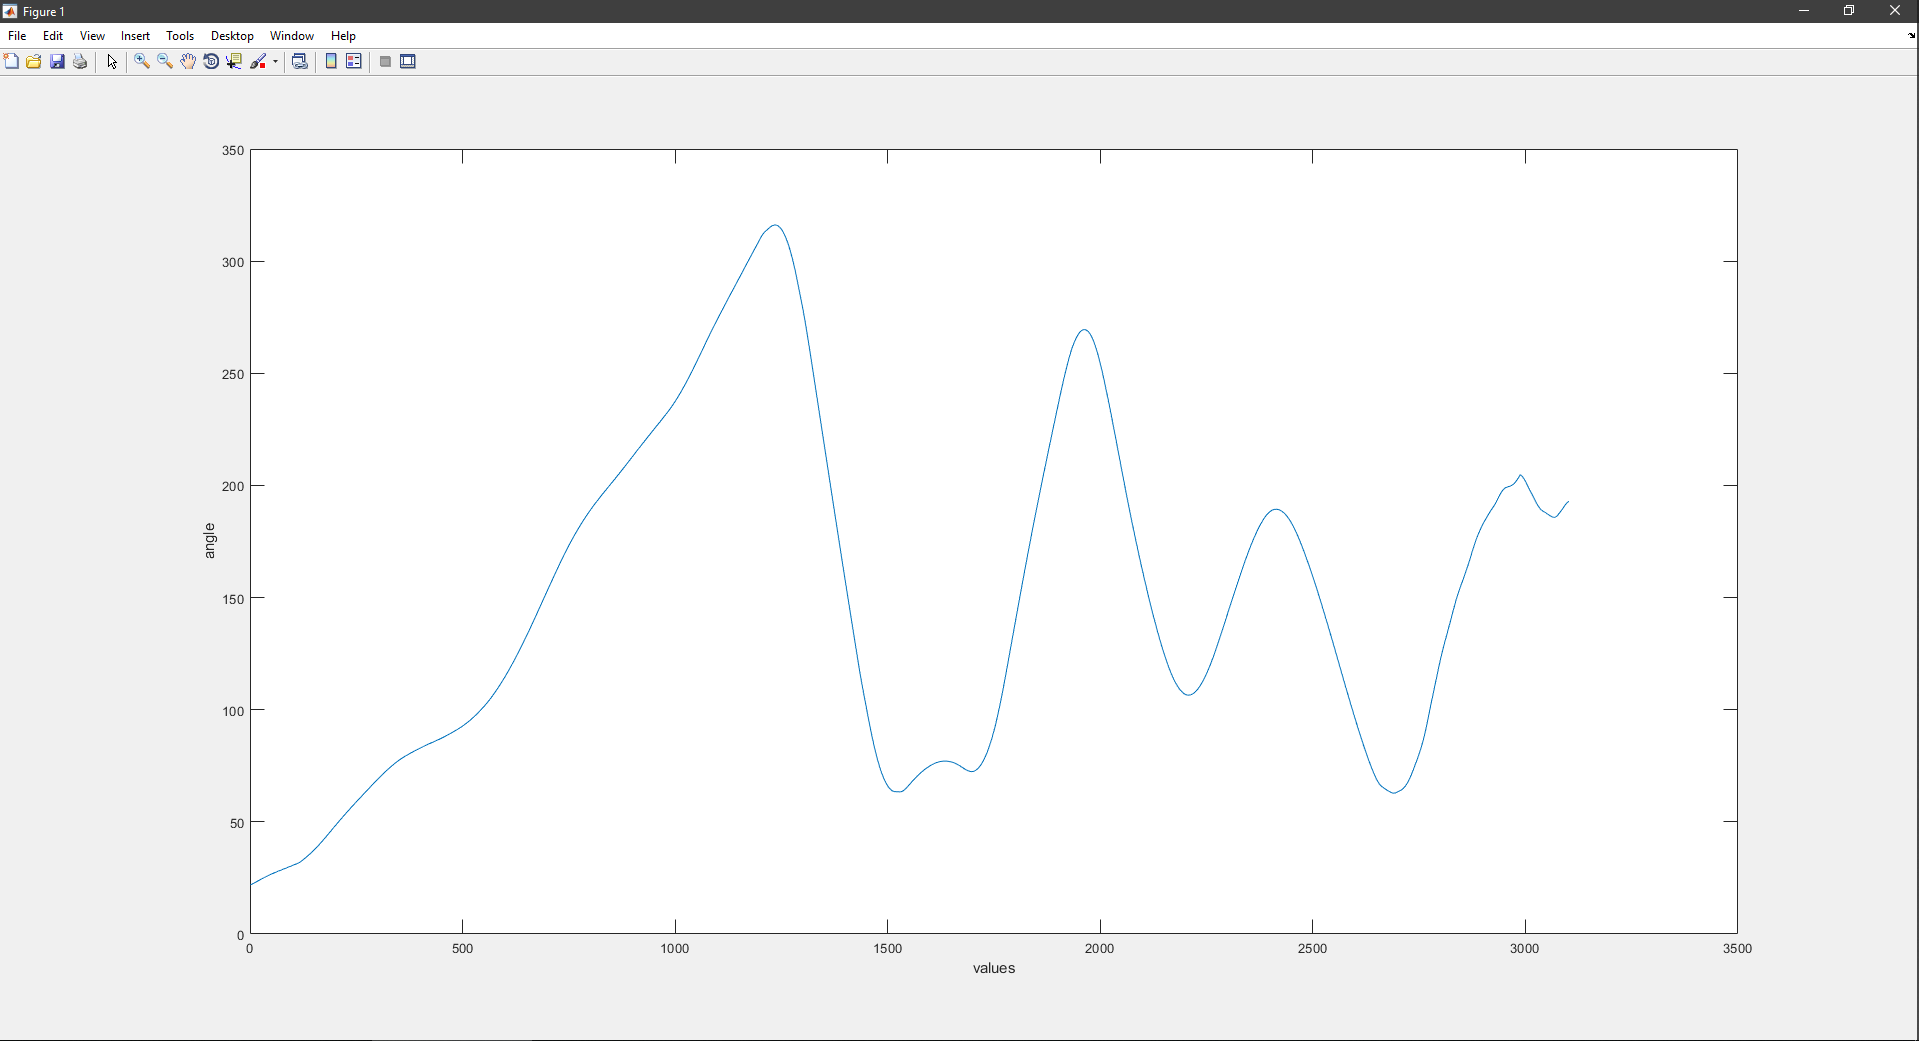
\includegraphics[scale=0.18]{Figuras/res_todos.png}
\caption{Valores obtidos com todos os anéis a comunicar}
\label{todos}
\end{figure}




